\documentclass{article}
\usepackage{graphicx}
\usepackage{amsmath}
\usepackage{url}

\title{Spirograph}
\author{Nishka Kacheria}
\date{October 2023}

%% \blurb{Spirographs are something we've played with since we were kids, with two gears inside of each other.}

\begin{document}

\maketitle

\section{Introduction}
\begin{center}
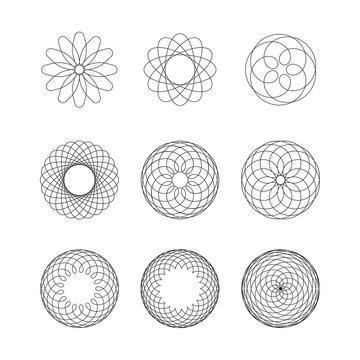
\includegraphics[width=4in]{images/Spirograph Examples.jpg}
\end{center}

Spirographs are something we've played with since we were kids, with two gears inside of each other. After placing your pencil in one of the gears, you would rotate the inner gear along the inner edge of the outer gear.

An example is shown here:

\begin{center}
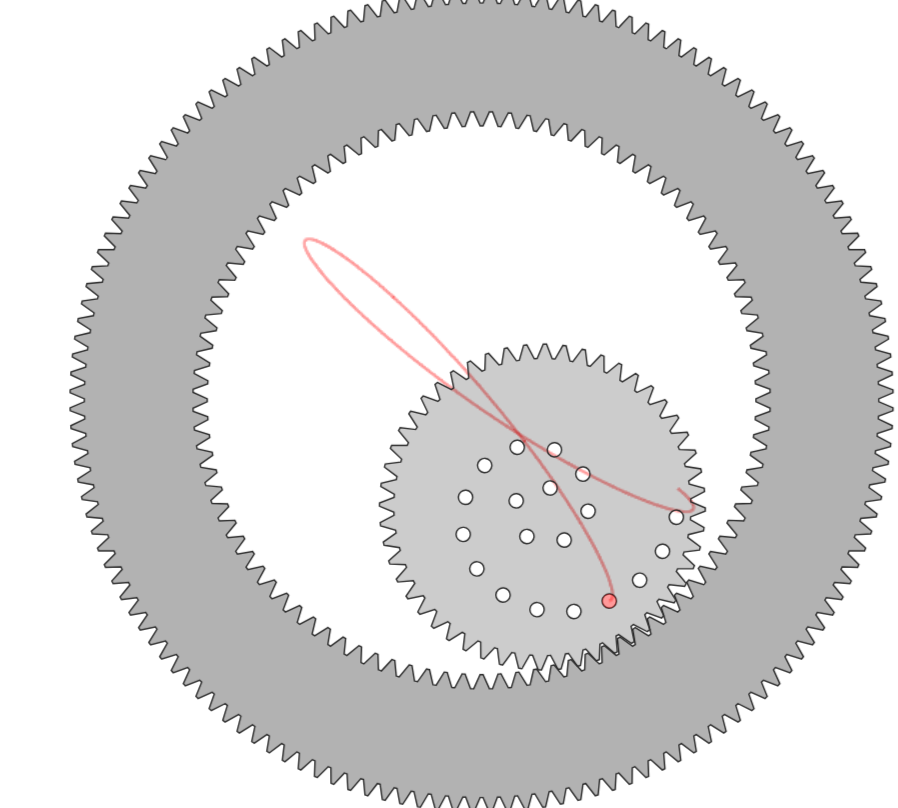
\includegraphics[width=4in]{images/Spirograph Example.png}
\end{center}

There are two things we can change. We can ch2ange the number of teeth in the inner gear, and the distance from the center of the circle of the point where our pencil is located in the inner gear.

The first thing to note is that when the pencil is located at the center of the smaller gear, it would create a circle (obviously).

However, when we start increasing the radius of the pencil on the inner circle, we get a new type of diagram. 

\begin{center}
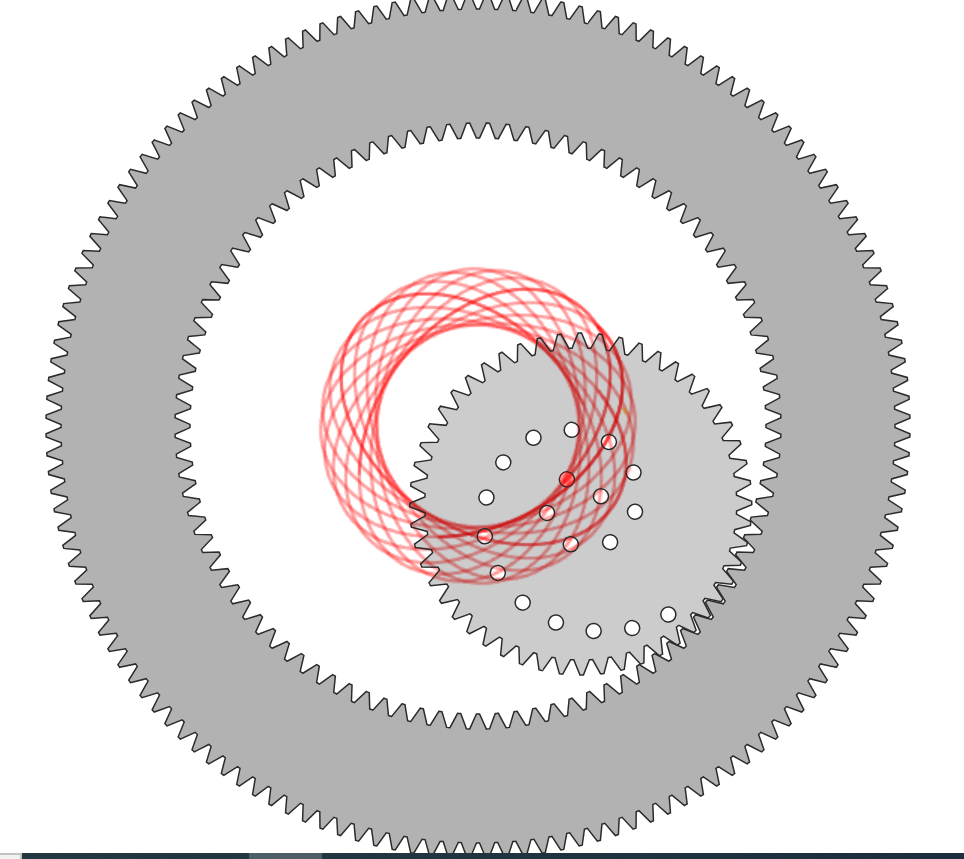
\includegraphics[width=4in]{images/IncreaseRad1.png}
\end{center}

Increasing the radius even more, we get 

\begin{center}
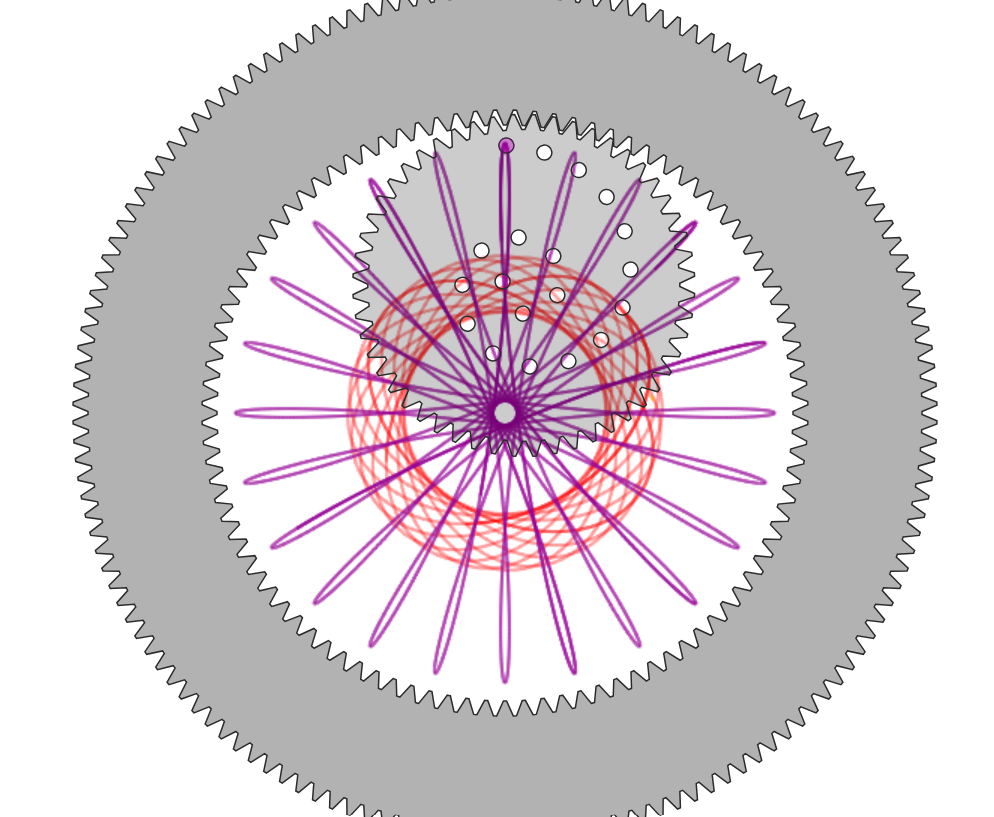
\includegraphics[width=4in]{images/MaxRad2.png}
\end{center}

In terms of intuition, it seems as though when the radius of pen at the inner gear increases, the spirograph becomes less circular and begins to form spokes.

\section{Spokes}

First, we can look at the number of spokes. We can define a spoke as one loop, and they are clearly distinct. Spokes also indicate another degree of symmetry.

The following example is a 32 tooth gear inside of a 96 toothed gear, with a variety of different inner radii, getting the following result. 

\begin{center}
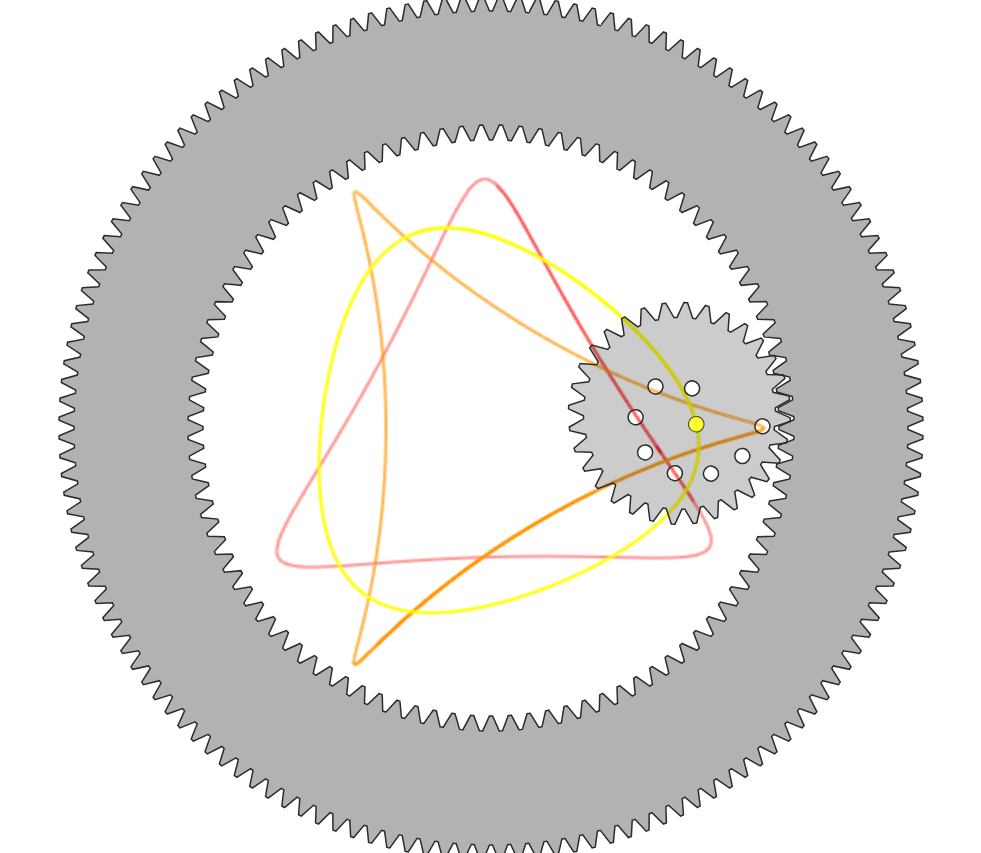
\includegraphics[width=4in]{images/Spokes.png}
\end{center}

The most obvious trend is that there are three spokes (or three points on the edges of the triangle). Perhaps this could be due to the fact that $32 * 3 = 96.$

We could continue looking at this with an inner-toothed gear with $64$ gears. 

\begin{center}
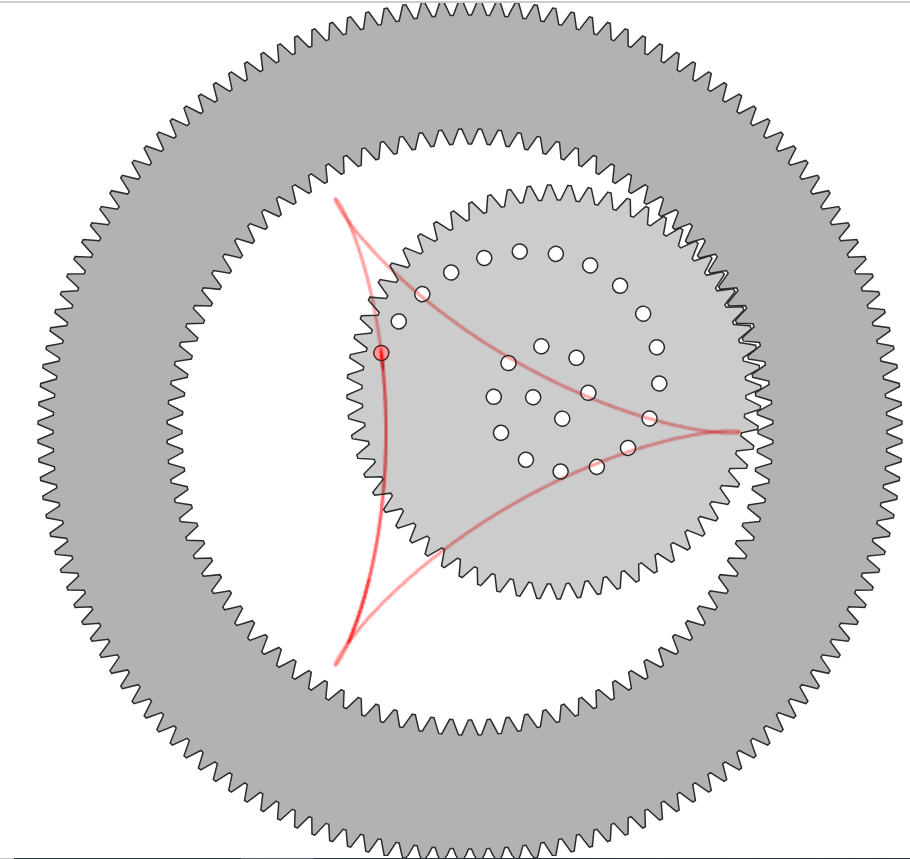
\includegraphics[width=4in]{images/Gear72.png}
\end{center}

This also had $3$ spokes. 

The next piece of intuition comes from the idea that $\frac{64}{96}$ is equal to $\frac{2}{3},$ which still has a denominator of $3.$

We can generalize this to a formula saying that the number of loops or spikes or degrees of symmetry is equal to the $\frac{\text{lcm}(r_1, r_2)}{r_2}$ where $r_1$ is the number of teeth in the outer gear and $r_2$ in the inner gear.

To explain this, note that each revolution of the inner gear creates a new loop. When the end of the new loop coincides with the beginning of the first loop, the rotation is complete. Then, imagine cutting open both of the circles and laying them flat on the same line. The number of times the inner gear repeats to make the outer gear is the number of revolutions. 

Thus, we can guess at the shape of a spirograph based solely on the gear sizes. 

Credit to \url{https://nathanfriend.io/inspiral-web} for the beginning diagrams.

\section{Spirograph}

First, note that the rotation matrix for plotting a circle based on the unit circle (so in a case where the inner radius is $0$) would be 

\begin{align*}
    x = \cos(\theta) - \sin(\theta) \\
    y = \sin(\theta) + \cos(\theta)
\end{align*}

However, we want to plot a point on the inner circle, not the outer circle. As a result, we can multiply the values of $x$ and $y$ by their distance from the origin, which would be $r_1 - r_2$ from the below diagram. 

\begin{center}
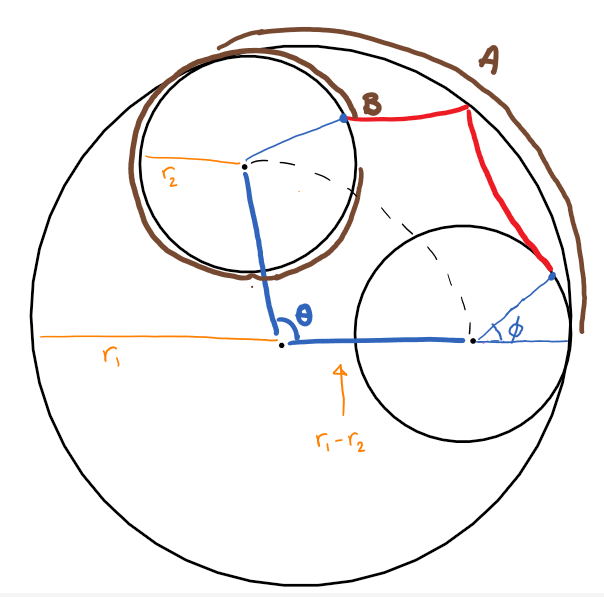
\includegraphics[width=4in]{images/Angle Diagram (1).png}
\end{center}

So the system of equations for the smaller circle is 
\begin{align*}
    x = (r_1 - r_2) \left( \cos(\phi) - \sin(\phi) \right)\\
    y = (r_1 - r_2) \left( \sin(\phi) + \cos(\phi) \right)
\end{align*}

The pen is the red path drawn. 

Further, when we look at just the inner gear, the pen is moving in a circle with angle $\phi.$ However, it is also moving around with radius $r_2$ relative to the center of the inner circle. 

As a result, we can add in the inner movement of the first gear. 

So, the new point's parametric equations are 
\begin{align*}
    x_i = r_2 \left( \cos(\phi) - \sin(\phi) \right) \\
    y_i = r_2  \left( \sin(\phi) + \cos(\phi) \right) \\
\end{align*}

Then, we can subtract the second set of equations from the first to get the location of the pen; 

\begin{align*}
    x = (r_1 - r_2) \left(\cos(\theta) - \sin(\theta) \right) - r_2  \left( \cos(\phi) - \sin(\phi) \right) \\
    y = (r_1 - r_2)(\sin(\theta) + \cos(\theta)) + r_2 (\sin(\phi) + \cos(\phi))
\end{align*}

To complete this, we want to find a way to relate $\theta$ to $\phi,$ where both are in terms of radians.

We can do that through noticing that the total distance travelled in terms of teeth for the inner gear and the outer gear is the same, or in other words, arcs A and B are the same length.

Thus, we can say that arc A, expressed as $r_1 \theta,$ is equal to arc B, or $r_2 (\theta + \phi).$ We have to add $\theta$ to the measurement of $B$ because the pen was not the only part that was moving, so was the gear itself. 

Then, we have $$r_1 \theta = r_2 (\theta + \phi)$$

Or $$ \phi = \frac{r_1 - r_2}{r_1}  \theta$$

Now we can plug these in and we have parametric equations that represent spirographs!

\begin{align*}
    x = (r_1 - r_2) (\cos(\theta) - \sin(\theta)) - r_2  \left( \cos\left(\frac{r_1 - r_2}{r_1}  \theta \right) - \sin\left(\frac{r_1 - r_2}{r_1}  \theta \right) \right) \\
    y = (r_1 - r_2) \left(\sin(\theta) + \cos(\theta) \right) + r_2 \left(\sin\left(\frac{r_1 - r_2}{r_1}  \theta \right) + \cos\left(\frac{r_1 - r_2}{r_1}  \theta \right) \right) \\
\end{align*}

Now that we have our parametric equations, we can graph spirographs, as shown below.

\begin{center}
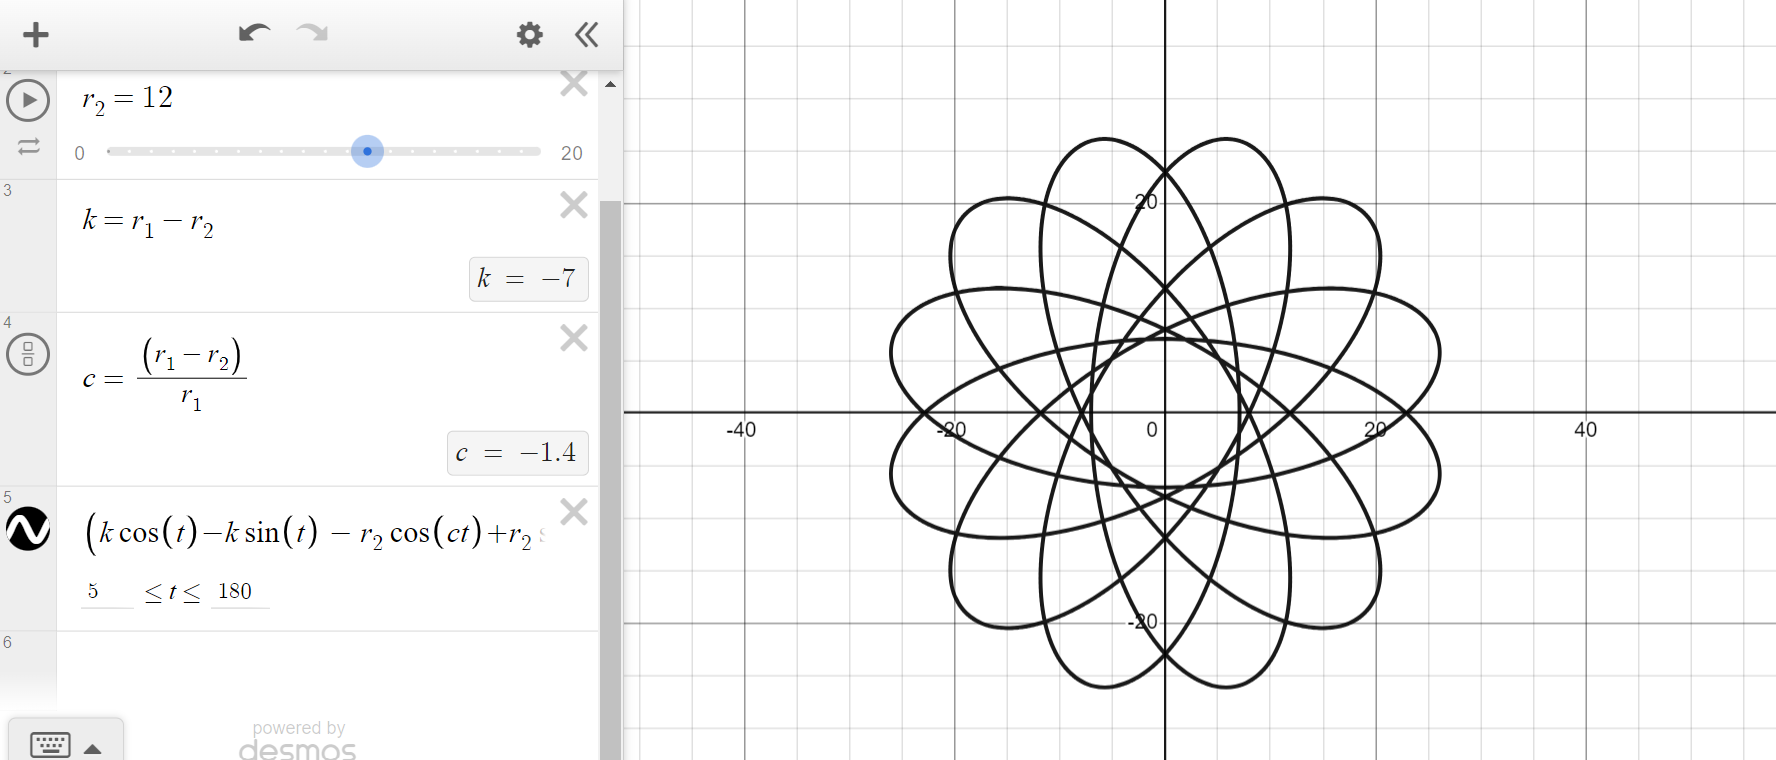
\includegraphics[height=5cm]{images/Spirograph.png}
\end{center}

Then, to simulate three gears, we can repeat the exact same process again. 

Note that from the perspective of the inner gear in our two diagram setup, the same process occurs with the smaller gear. As a result, we can write that for the inner gear, it's equations are 

\begin{align*}
    x = (r_2 - r_3) (\cos(\phi) - \sin(\phi)) - r_3  \left( \cos\left(\frac{r_2 - r_3}{r_2}  \phi \right) - \sin\left(\frac{r_2 - r_3}{r_2}  \phi \right) \right) \\
    y = (r_2 - r_2) \left(\sin(\phi) + \cos(\phi) \right) + r_3 \left(\sin\left(\frac{r_2 - r_3}{r_2}  \phi \right) + \cos\left(\frac{r_2 - r_3}{r_2}  \phi \right) \right) \\
\end{align*}

Then, we can add this back to our initial set of equations, but negative. This also makes sense because the third gear would be rotating in the same direction as the first, outer gear, so it should be added back to the overall equation. 

Additionally, note that this is $\phi.$ Substituting in $\theta$ for $\phi$ using te equations we previously had, we get
\[
\begin{aligned}
    x &= k\cos\left(t\right)-k\sin\left(t\right)\ -k_{2}\cos\left(ct\right)+k_{2}\sin\left(ct\right) + r_{3}\cos\left(c \cdot c_{2}t\right)-r_{3}\sin\left(c \cdot c_{2}t\right) \\
    y &= k\sin\left(t\right)+k\cos\left(t\right) -k_{2}\sin\left(ct\right)-k_{2}\cos\left(ct\right)+r_{3}\sin\left(c \cdot c_{2}t\right)+r_{3}\cos\left(c\cdot c_{2}t\right)
\end{aligned}
\]
Where $k = \frac{r_1 - r_2}{r_1},$ and $k_2 = \frac{r_2 - r_3}{r_2},$ $c = \frac{r_1 - r_2}{r_1},$ and $c_2 = \frac{r_2 - r_3}{r_2}$.

This gives

\begin{center}
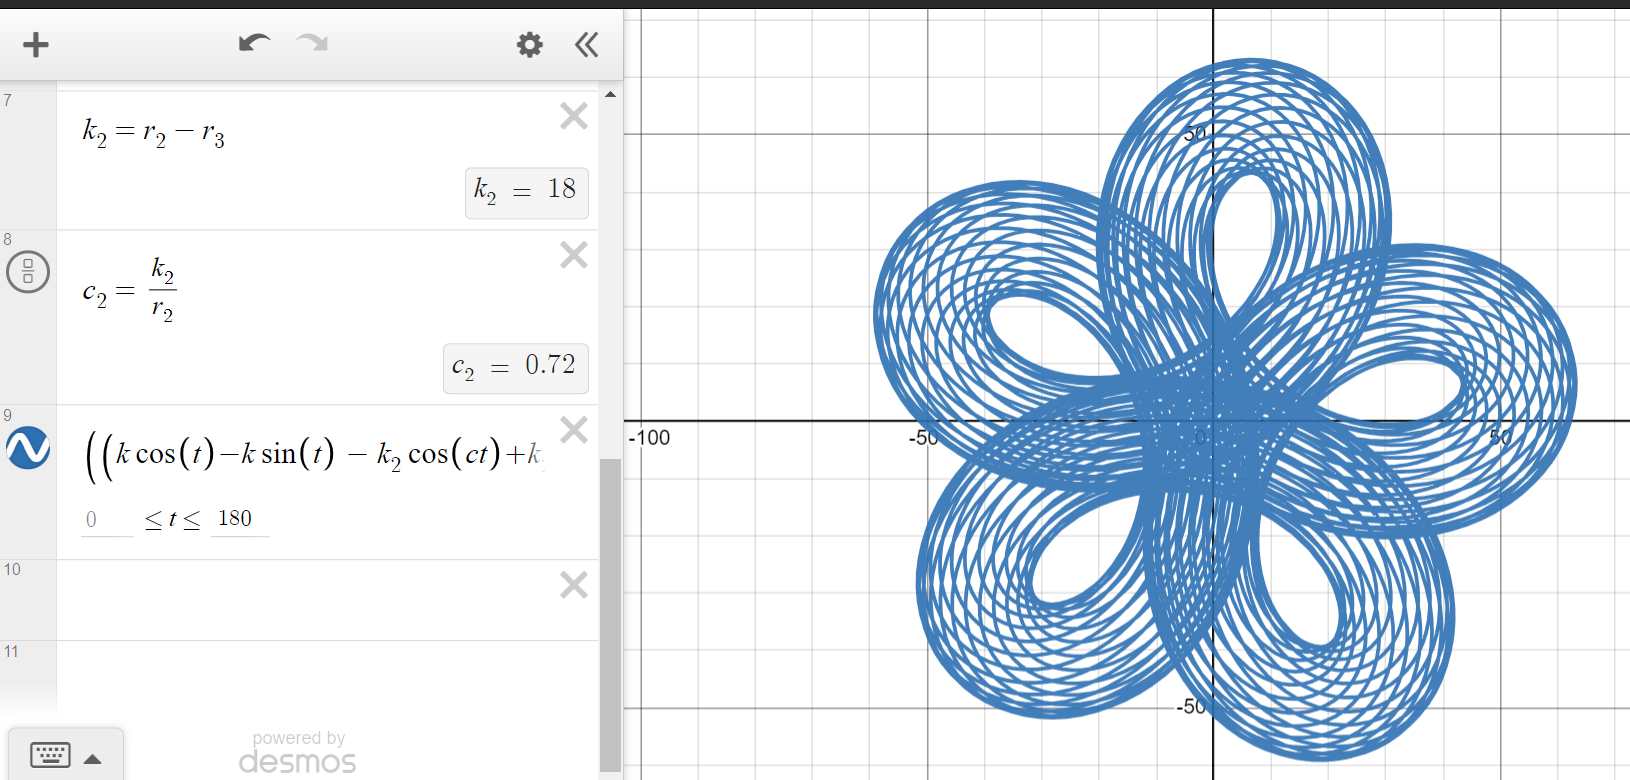
\includegraphics[height=5cm]{images/3-Gear Spiro.png}
\end{center}

We can continue extrapolating this process to get 4 and any number of gear spirographs. 

Here is a four gear spirograph, similarly derived.

\begin{center}
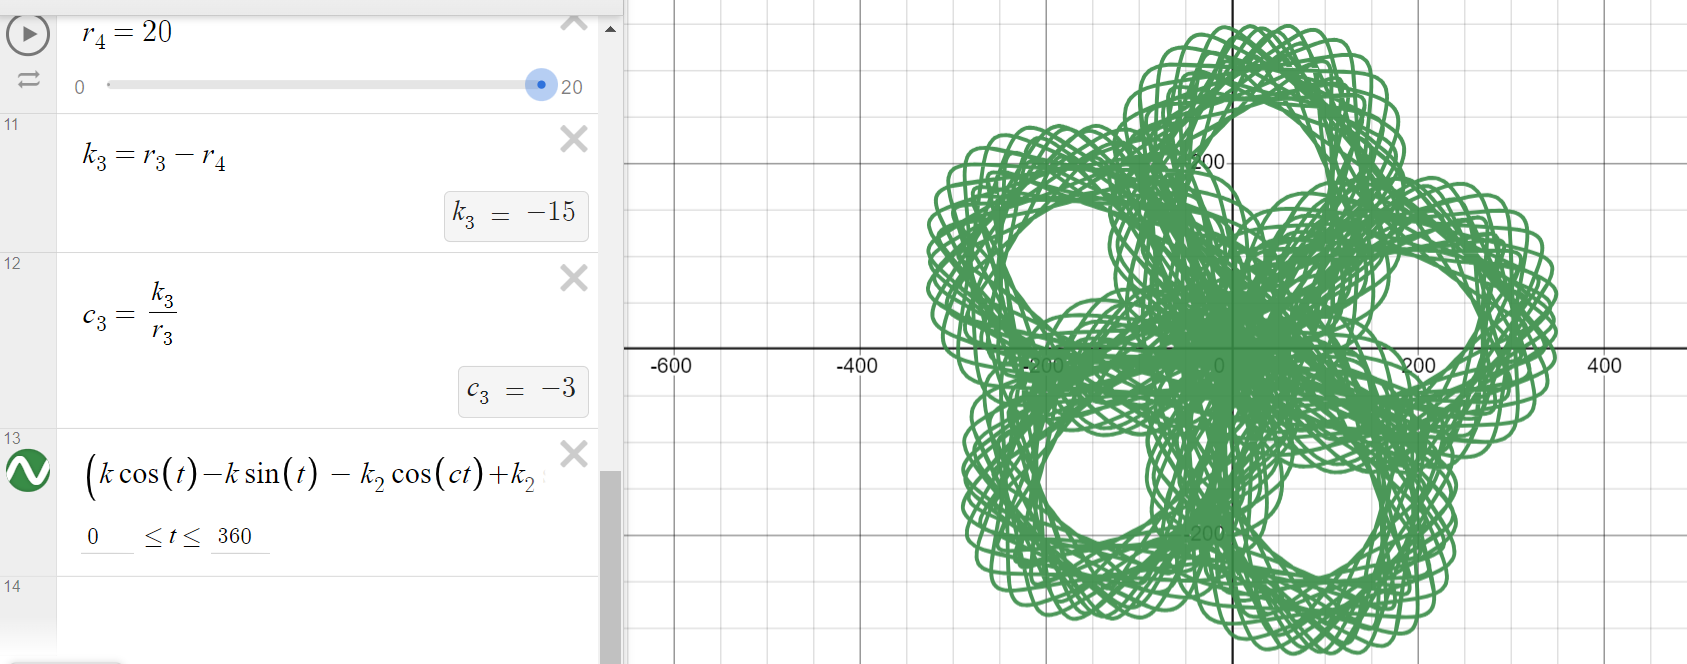
\includegraphics[height=5cm]{images/4 Gear Spiro.png}
\end{center}

Its equations are
\begin{align*}
    x = &\ k\cos\left(t\right)-k\sin\left(t\right)\ -\\
        &\ k_{2}\cos\left(ct\right)+k_{2}\sin\left(ct\right)\ +\\
        &\ k_{3}\cos\left(cc_{2}t\right) - k_{3}\sin\left(cc_{2}t\right)\ -\\
        &\ r_{4}\cos\left(cc_{2}c_{3}t\right)+r_{4}\sin\left(cc_{2}c_{3}t\right) \\
    y = &\ k\sin\left(t\right)+k\cos\left(t\right)\ -\\
        &\ k_{2}\sin\left(ct\right) - k_{2}\cos\left(ct\right) +\\
        &\ k_{3}\sin\left(cc_{2}t\right) + k_{3}\cos\left(cc_{2}t\right)-& \\
        &\ r_{4}\sin\left(cc_{2}c_{3}t\right)-r_{4}\cos\left(cc_{2}c_{3}t\right) \\
\end{align*}
We can keep going, making 5, 6, and more geared spirographs.

\end{document}

  